\documentclass[12pt]{article}
\usepackage[utf8]{inputenc}
\usepackage{polski}
\usepackage{indentfirst}
\usepackage{graphicx}

\title{Obliczenia Naukowe \\ \large Lista nr 3}
\author{Eryk Krupa \\ 244993}
\date{}

\begin{document}
\renewcommand{\familydefault}{\sfdefault}
\maketitle
\newpage

\section{Zadanie 1, 2 i 3}
Poniższe rozważania dotyczą trzech algorytmów wyznaczania przybliżonej wartości pierwiastka funkcji:
\begin{itemize}
    \item metoda bisekcji,
    \item metoda stycznych,
    \item metoda siecznych.
\end{itemize}

\subsection{Metoda Bisekcji}
\subsubsection{Opis}
Algorytm na wejściu przyjmuje dwie wartości: początek ($a$) i koniec ($b$) przedziału, w którym szukane będzie miejsce zerowe. By działał poprawnie, muszą być spełnione dwa warunki. Wartości funkcji na końcach przedziałów muszą mieć różne znaki, tj. $f(a)f(b)<0$ oraz funkcja w tym przedziale musi być ciągła.
\begin{figure}[!htbp]
    \centering
    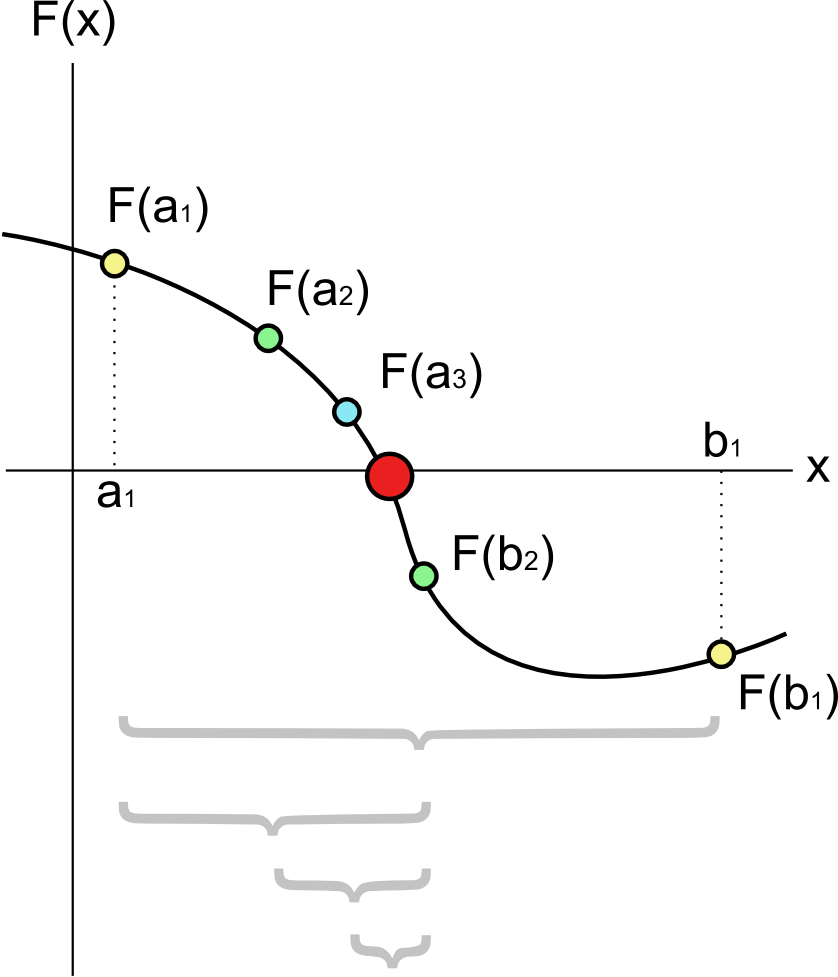
\includegraphics[height=150px]{bisection_method.png}
    \caption{Metoda bisekcji}
    \label{fig:bisection}
\end{figure}
\subsubsection{Przebieg}
Początkowo obliczana jest długość przedziału $length=b-a$. Następnie dzielona jest przez dwa i dodawana do wartości a:  $middle=a+length$. Jeśli przedział jest mniejszy od początkowo przyjętej dokładności, algorytm zwraca punkt middle oraz wartość funkcji $f(middle)$ w punkcie. W przeciwnym wypadku, przedział dzielony jest na dwa mniejsze przedziały $[a, middle]$ oraz $[middle, b]$. Następnie algorytm podstawia pod a i b odpowiednio początek i koniec przedziału, w którym wyniki funkcji na jego końcach mają różne znaki.

\subsection{Metoda stycznych}
\subsubsection{Opis}
Metoda stycznych znana jest również pod nazwą metody Newtona. By algorytm działał poprawnie, pierwiastek musi być jednokrotny tj. $f'(r)\neq0$. Ponadto, musi zostać obrany punkt startowy $x_0$.
\begin{figure}[!htbp]
    \centering
    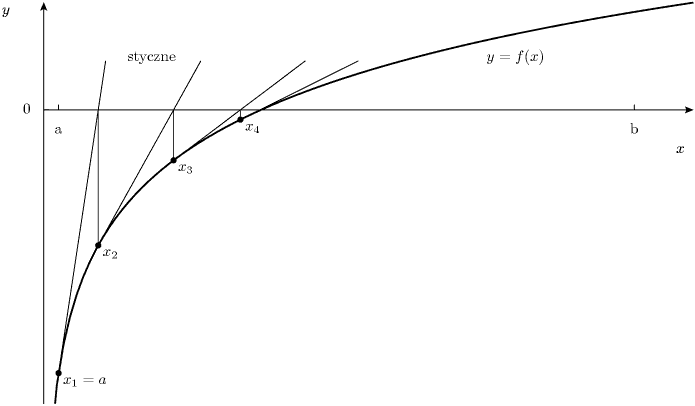
\includegraphics[height=150px]{newton_method.png}
    \caption{Metoda stycznych}
    \label{fig:tangent}
\end{figure}
\subsubsection{Przebieg}
Każdy kolejny punkt $x_{n+1}$ obliczany jest na podstawie wzoru $$x_{n+1}=x_n-\frac{f(x_n)}{f'(x_n)}.$$ Następnie obliczana jest wartość funkcji $f(x_{n+1})$. Obliczenia są kończone, kiedy znalezione wartość $f(x_{n+1})$ jest na tyle bliska zeru, że $|f(x_{n+1})|$ jest mniejsze od pewnej ustalonej dokładności, bądź też odległość pomiędzy kolejnymi wartościami $x_{n+1}$ i $x_n$ jest dostatecznie mała.

\subsection{Metoda siecznych}
\subsubsection{Opis}
By algorytm działał poprawnie, pierwiastek musi być jednokrotny tj. $f'(r)\neq0$. Ponadto, muszą zostać podane dwa przybliżenia początkowe $x_0$ i $x_1$.
\begin{figure}[!htbp]
    \centering
    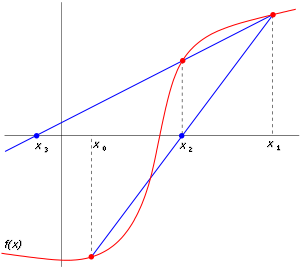
\includegraphics[height=150px]{secant_method.png}
    \caption{Metoda siecznych}
    \label{fig:secant}
\end{figure}
\subsubsection{Przebieg}
W przypadku metody siecznych również korzystamy z pochodnej funkcji, jednak w odróżnieniu od metody stycznych, jest ona aproksymowana za pomocą wzoru: $$f'(x_n)\approx\frac{f(x_n)-f(x_{n-1})}{x_n-x_{n-1}}.$$ Dopiero tak obliczoną pochodną podstawiamy do wzoru z metody stycznych, otrzymując $$x_{n+1}=x_n-f(x_n)\frac{x_n-x_{n-1}}{f(x_n)-f(x_{n-1})}.$$
Tu właśnie widać, dlaczego metoda siecznych wymaga dwóch przybliżeń początkowych. W każdej iteracji $x_{n+1}$ wymaga $x_n$ i $x_{n-1}$.

\subsection{Porównanie metod}
Największą wadą metody bisekcji jest to, że należy sprecyzować dla niej przedział, na którym spodziewamy się znaleźć miejsce zerowe. W pozostałych metodach nie ma takiego wymagania. Co prawda, należy wskazać przybliżenia początkowe (lub przybliżenia, w metodzie siecznych), ale tylko po to, by przyśpieszyć działania algorytmu przez zmniejszenie liczby iteracji. Jeśli podane przybliżenie początkowe jest odległe od rzeczywistej wartości, algorytm i tak znajdzie prawidłowe rozwiązanie, jednak zajmie mu to więcej iteracji. W przypadku metody Newtona można zauważyć inny problem- jeśli pochodna rozpatrywanej funkcji w punkcie podanym jako przybliżenie początkowe jest bliska zeru, nie można w prawidłowy sposów wyznaczyć miejsca zerowego.

\section{Zadanie 4}
\subsection{Wyniki}
Pierwiastek równania $sin(x) - (\frac{1}{2}x)^2 = 0$ obliczony za pomocą trzech powyższych metod:

\begin{center}
\begin{tabular}{ |c|c|c|c| }
\hline
Metoda & $x_0$ & $sin(x_0) - (\frac{1}{2}x_0)^2 = 0$ & iteracje\\ \hline
bisekcji & 1.9337539672851562 & -2.7027680138402843e-7 & 16 \\
stycznych & 1.933749984135789 & 4.995107540040067e-6 & 13\\
siecznych & 1.9337539405015145 & -2.3487103129049558e-7 & 5\\ \hline
\end{tabular}
\end{center}

\subsection{Opis}
Można zauważyć, że każda z metod znajduje niemal identyczne miejsce zerowe. Różnica widoczna jest natomiast w ilości iteracji. Widać, że metoda bisekcji jest najwolniejsza, a metoda siecznych- najszybsza. Były to wyniki oczekiwane, zgodne z wydajnością tych algorytmów. Należy jednak pamiętać, że w przypadku innej funkcji mogłoby być inaczej- teoretycznie najwolniejszy algorytm bisekcji mógłbym zakończyć pracę w ilości iteracji mniejszej od pozostałych algorytmów.

\section{Zadanie 5}
Znajdźmy wartości zmiennej x, dla której funkcje $f_1(x) = 3x$ oraz $f_2(x) = e^x$ przecinają się.
\subsection{Rozwiązanie}
Oczywiście, najprostrzym rozwiązaniem jest policzenie miejsc zerowych różnicy tych funkcji $f_3(x) = f_2(x)-f_1(x) = e^x-3x$, oznaczonej na wykresie kolorem zielonym. $f_1(x)$ oznaczone jest kolorem czerwonym, natomiast $f_2(x)$ - niebieskim.
\begin{figure}[!htbp]
    \centering
    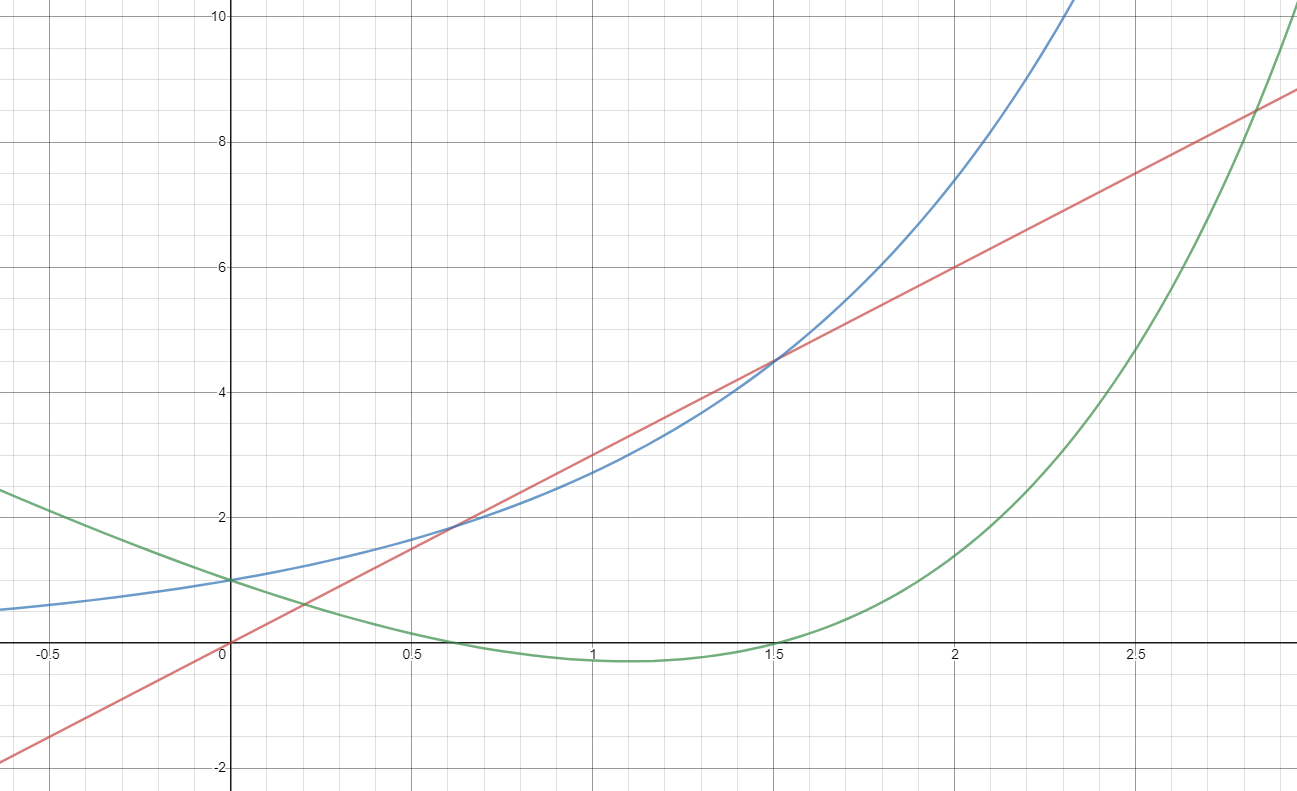
\includegraphics[width=380px]{graph.png}
    \caption{Wykres}
    \label{fig:secant}
\end{figure}
\subsection{Wyniki}
Używając metody bisekcji na odpowiednich przedziałach, np. na [0, 1] i [1, 2], możemy za jej pomocą odnaleść oba miejsca zerowe.
\begin{center}
\begin{tabular}{ |c|c|c|c| }
\hline
Przedziały & $x_0$ & $f(x_0)$ & iteracje\\ \hline
$[0, 1]$ & 0.619140625 & 9.066320343276146e-5 & 9\\
$[1, 2]$ & 1.5120849609375 & 7.618578602741621e-5 & 13\\ \hline
\end{tabular}
\end{center}
Funkcje przecinają się w dwóch miejscach. W przypadku metody bisekcji, może okazać się to problematyczne, chyba, że jesteśmy w stanie w przybliżeniu określić w jakich przedziałach znajdują się miejsca zerowe. W naszym przypadku, dzięki zastosowanemu wykresowi było to proste, jednak gdybyśmy nie znali przybliżonych pozycji miejsc zerowych, musielibyśmy trochę poeksperymentować, aby trafić na przedział, na którego końcach znajdują się wartości o różnych znakach. Gdybyśmy dla przykładu wzieli przedział [0, 2],  nie moglibyśmy jednoznacznie określić nawet, czy pomiędzy nimi znajdują się miejsca zerowe, czy nie, gdyż wartości na końcach tego przedziału mają taki sam znak.

\section{Zadanie 6}
Znajdźmy miejsca zerowe funkcji $f_1(x) =e^{(1-x)}-1$ oraz $f_2(x) = xe^{-x}$ za pomocą trzech wyżej wymienionych metod, przyjmując precyzję $\delta=10^{-5}$ oraz $\epsilon=10^{-5}$.
\subsection{Wyniki}

\subsubsection{Funkcja $e^{(1-x)}-1$}
\begin{center}
\begin{tabular}{ |c|c|c|c| }
\hline
Metody & Przedział lub & Miejsce zerowe & Wartość funkcji\\ 
 & punkt(y) początkowy/e & & \\ \hline
bisekcji & $[0, 2]$ & 1.0 & 0.0\\
stycznych & 1.0 & 1.0 & 0.0\\
siecznych & 0, 2 & 0.99999961170  & 3.8829645854e-7\\ \hline
\end{tabular}
\end{center}

\subsubsection{Funkcja $xe^{-x}$}
\begin{center}
\begin{tabular}{ |c|c|c|c| }
\hline
Metody & Przedział lub & Miejsce zerowe & Wartość funkcji\\ 
 & punkt(y) początkowy/e & & \\ \hline
bisekcji & $[-1, 1]$ & 0.0 & 0.0\\
stycznych & 0.0 & 0.0 & 0.0\\
siecznych & -0.1, 0.1 & -9.5487043590e-6 & -9.5487955371e-6\\ \hline
\end{tabular}
\end{center}
 
\subsection{Analiza}
W tabelach przedstawiono idealne sytuacje, dla których łatwo można obliczyć miejsca zerowe. Dla przykładu, w przypadku metody bisekcji można znaleźć miejsce zerowe w jednej iteracji, jeśli znajduje się ono dokładnie na środku przedziału. W przypadku metody Newtona, najlepsza sytuacja to taka, w której 
miejscem zerowym okazuje się punkt początkowy.

W przypadku funkcji $e^{(1-x)}-1$ z metodą Newtona dla $x_0 \in (1, \infty]$ można zauważyć, że im bardziej oddalamy się od miejsca zerowego, tym większej ilości iteracji potrzebujemy, aby poprawnie je wyznaczyć.

Z kolei funkcja  $xe^{-x}$ dla $x_0>1$ przyjmuje wartości bardzo bliskie zeru, dlatego metoda Newtona znajduje miejsce zerowe niemal wszędzie, w pierwszej iteracji. W przypadku wybrania wartości początkowej równej 1.0, pochodna z tej funkcji, tj. $-e^{-x}(x-1)$ wynosi zero, dlatego też algorytm Newtona przerwie wykonania z odpowiednim błędem. 

\end{document}
